\documentclass{beamer}
\usepackage[utf8]{inputenc}
\usetheme{Warsaw}

\title[Slovenski NLTK označevalnik]{Slovenski NLTK označevalnik}
\author{
	Niko Colnerič
	\and
	Nejc Banič}
\institute{ Fakulteta za Računalništvo in Informtiko\\
			Univerza v Ljubljani}

\begin{document}

\begin{frame}
\titlepage
\end{frame}

\begin{frame}{Motivacija}
\begin{itemize}
\item NLTK - Natural Language Toolkit (Python 2.7)
\item Označevalnik (tagger) besedam pripiše oblikoslovne oznake
\item Težave z dvoumnostjo
\item Uporabnost za nadaljno procesiranje teksta
\item Tega so nas učili v šoli $\ddot\smile$
\end{itemize}
\end{frame}

\begin{frame}{Implementirani označevalniki}
\begin{itemize}
\item \textbf{Trigram označevalnik}\\
\textit{a priori najbolj verjetno oznako v kontekstu dolžine 3}
\begin{center}
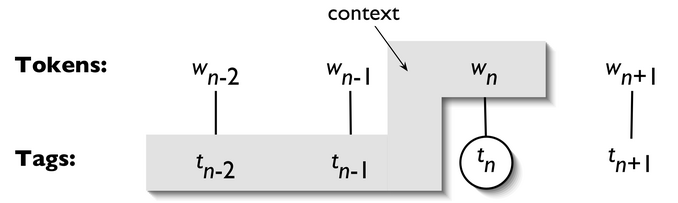
\includegraphics[width=0.6\textwidth]{../paper/tag-context.png}
\end{center}

\item \textbf{Brillov označevalnik}\\
\textit{ugane oznako vsako besede, nato 
popravi svoje napake tako, da uporabi seznam transformacijskih pravil}
\item označevalnik na podlagi \textbf{naivnega Bayes-ovega klasifikatorja}\\
\textit{predpostavi pogojno neodvisnost atributov pri danem razredu}
\end{itemize}
\end{frame}

\begin{frame}{JOS korpus}
\begin{itemize}
\item korpus = velika in strukturirana zbirka besedil
\item Jezikoslovno Označevanje Slovenskega jezika (IJS)
\item Zbirko besedil s ročno preverjenimi jezikoslovnimi oznakami
\item \textit{.XML} datoteka
\item Uporabila sva \textit{jos1M} - 1 milijon označenih besed
\item MULTEXT-East V4 specifikacija
\item MSD (morphosyntactic descriptions) - definirajo kategorije oz. besedne vrste
\item Namenjena spodbujanju razvoja jezikovnih tehnologij za slovenski jezik
\end{itemize}
\end{frame}

\begin{frame}{NLTK trainer}
\begin{itemize}
\item Uporabljen za treniranje NLTK objektov - označevanlikov
\item \textit{Train NLTK objects with zero code}
\item Dobro dokumentiran
\item Prosto dostopen na Github-u
\end{itemize}
\end{frame}

\begin{frame}{Postopek treniranja označevalnikov}
\begin{enumerate}
\item Transformacija \textit{.XML} korpusa v \textit{.pos}
\item Treniranje z skripto iz NLTK-trainer
\item Ocenjevanje točnosti
\item Ocenjevanje hitrosti
\end{enumerate}
\end{frame}

\begin{frame}{Primer}
\begin{center}
\textit{\textbf{Lep je dan, vse diši že po pomladi!}}
\end{center}
\textit{( Lep  |  PPNMEIN ) - pridevnik\\
	( je  |  GP-STE-N ) - glagol\\
	( dan  |  SOMEI ) - samostalnik\\
	( ,  |  , ) - ni razlage\\
	( vse  |  ZC-SEI ) - zaimek\\
	( diši  |  GGNSTE ) - glagol\\
	( že  |  L ) - členek\\
	( po  |  DM ) - predlog\\
	( pomladi  |  SOZEM ) - samostalnik\\
	( !  |  ! ) - ni razlage}\\
\end{frame}

\begin{frame}{Celoten MSD za \textit{Lep} }
\begin{center}
\begin{tabular}{c|c}
\multicolumn{2}{c}{pridevnik}\\\hline\hline
vrsta & splošni \\
spol & moški \\
število & ednina \\
sklon & imenovalnik \\
živost & 0 \\
vid & 0 \\
oblika & 0 \\
oseba & 0 \\
nikalnost & 0 \\
stopnja & nedoločeno \\
določnost & ne \\
število\_svojine & 0 \\
spol\_svojine & 0 \\
naslonskost & 0 \\
zapis & 0 \\
\end{tabular}
\end{center}
\end{frame}

\begin{frame}{Rezultati natančnost}
\begin{figure}[h]
\begin{center}
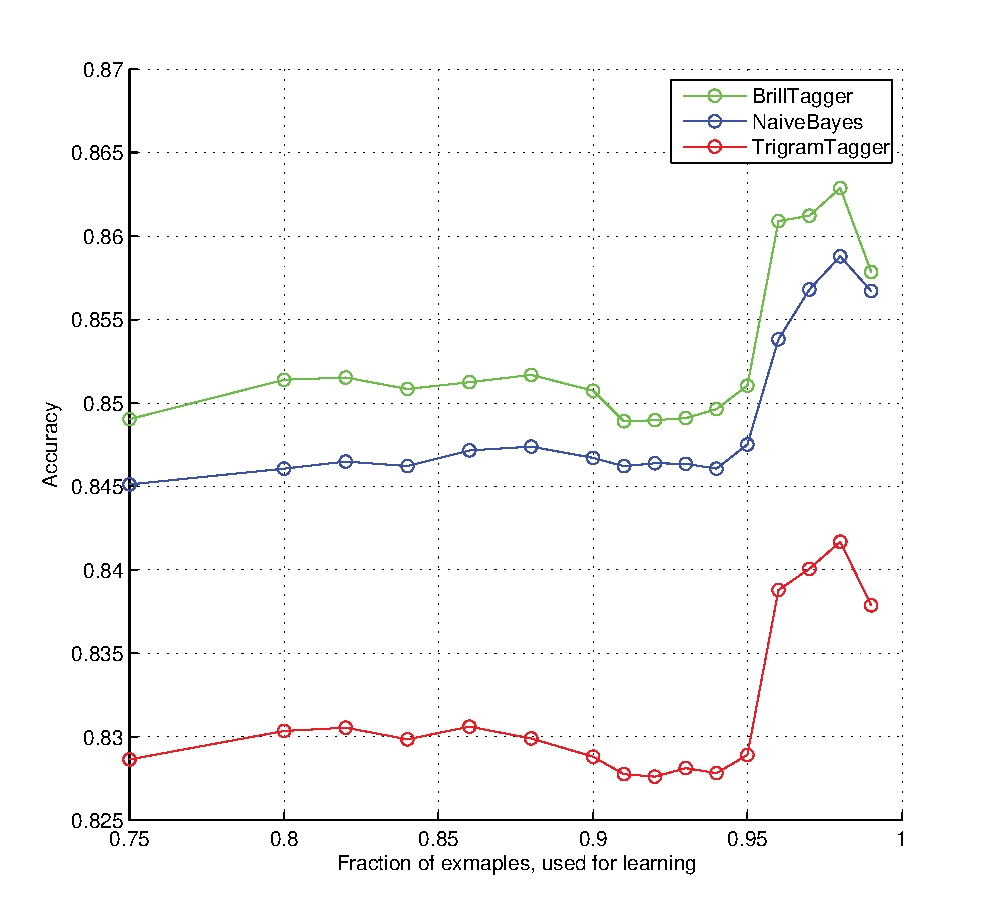
\includegraphics[height=0.85\textheight]{../evaluation/graph.pdf} 
\end{center}
\end{figure}
\end{frame}

\begin{frame}{Rezultati hitrost}
\begin{figure}[h]
\begin{center}
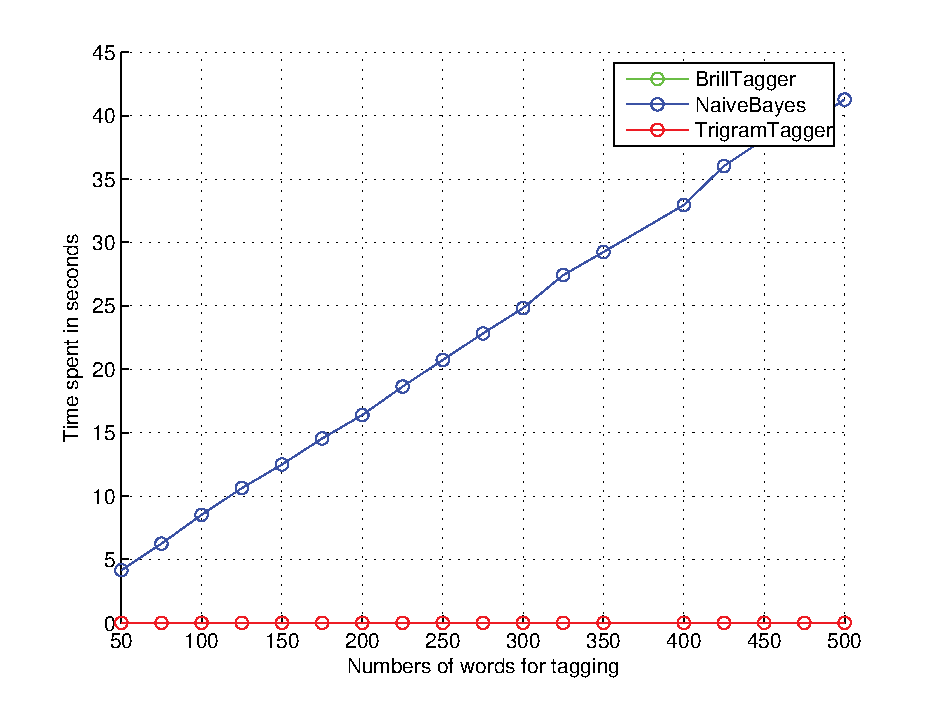
\includegraphics[height=0.85\textheight]{../evaluation/graph_speed.pdf} 
\end{center}
\end{figure}
\end{frame}

\begin{frame}{Zaključek, izboljšave}
\begin{itemize}
\item Brill in Trigram sta hitra, NaiveBayes veliko počasnejši
\item Najbolj natančen Brill, najmanj Trigram
\item $\Rightarrow$ Priporočama uporabo Brill označevalnika
\item Vključitev v NLTK
\item Dostopno na: \url{https://github.com/nikicc/slovene-nltk-tagger}
\end{itemize}
 
\begin{itemize}
\item Z lahkoto bi zgradili tudi druge označevalnike, ki bi lahko bili boljši ali hitrejši
\item Vključitev drugih korpusov, bi bila koristna
\end{itemize}
\end{frame}

\end{document}